\documentclass[a4paper,12pt]{article}
\usepackage[top = 2.5cm, bottom = 2.5cm, left = 2.5cm, right = 2.5cm]{geometry}
\usepackage[T1]{fontenc}
\usepackage[utf8]{inputenc}
\usepackage{multirow} 
\usepackage{booktabs} 
\usepackage{graphicx}
\usepackage[spanish]{babel}
\usepackage{setspace}
\setlength{\parindent}{0in}
\usepackage{float}
\usepackage{fancyhdr}
\usepackage{amsmath}
\usepackage{amssymb}
\usepackage{amsthm}
\usepackage[numbers]{natbib}
\newcommand\Mycite[1]{%
	\citeauthor{#1}~[\citeyear{#1}]}
\usepackage{graphicx}
\usepackage{subcaption}
\usepackage{booktabs}
\usepackage{etoolbox}
\usepackage{minibox}
\usepackage{hyperref}
\usepackage{xcolor}
\usepackage{pdfpages}
\usepackage[skins]{tcolorbox}
%---------------------------

\newtcolorbox{cajita}[1][]{
	 #1
}

\newenvironment{sol}
{\renewcommand\qedsymbol{$\square$}\begin{proof}[\textbf{Solución.}]}
	{\end{proof}}

\newenvironment{dem}
{\renewcommand\qedsymbol{$\blacksquare$}\begin{proof}[\textbf{Demostración.}]}
	{\end{proof}}

\newtheorem{problema}{Problema}
\newtheorem{definicion}{Definición}
\newtheorem{ejemplo}{Ejemplo}
\newtheorem{teorema}{Teorema}
\newtheorem{corolario}{Corolario}[teorema]
\newtheorem{lema}[teorema]{Lema}
\newtheorem{prop}{Proposición}
\newtheorem*{nota}{\textbf{NOTA}}
\renewcommand\qedsymbol{$\blacksquare$}
\usepackage{svg}
\usepackage{tikz}
\usepackage[framemethod=default]{mdframed}
\global\mdfdefinestyle{exampledefault}{%
linecolor=lightgray,linewidth=1pt,%
leftmargin=1cm,rightmargin=1cm,
}




\newenvironment{noter}[1]{%
\mdfsetup{%
frametitle={\tikz\node[fill=white,rectangle,inner sep=0pt,outer sep=0pt]{#1};},
frametitleaboveskip=-0.5\ht\strutbox,
frametitlealignment=\raggedright
}%
\begin{mdframed}[style=exampledefault]
}{\end{mdframed}}
\newcommand{\linea}{\noindent\rule{\textwidth}{3pt}}
\newcommand{\linita}{\noindent\rule{\textwidth}{1pt}}

\AtBeginEnvironment{align}{\setcounter{equation}{0}}
\pagestyle{fancy}

\fancyhf{}









%----------------------------------------------------------
\lhead{\footnotesize Data Science I}
\rhead{\footnotesize  Rudik Roberto Rompich}
\cfoot{\footnotesize \thepage}


%--------------------------

\begin{document}
 \thispagestyle{empty} 
    \begin{tabular}{p{15.5cm}}
    \begin{tabbing}
    \textbf{Universidad del Valle de Guatemala} \\
    Departamento de Ciencias de la Computación\\\\
   \textbf{Estudiantes:} Augusto Alonso, Angel Cuellar, Rudik Roberto Rompich\\
    \end{tabbing}
    \begin{center}
        CC3066 - Data Science I - Catedrático: Luis Furlan\\
        \today
    \end{center}\\
    \hline
    \\
    \end{tabular} 
    \vspace*{0.3cm} 
    \begin{center} 
    {\Large \bf  Proyecto 2 - Análisis Exploratorio 
} 
        \vspace{2mm}
    \end{center}
    \vspace{0.4cm}
%--------------------------

\textbf{Instrucciones:} 

Para este ejercicio, trabajarán con 4 conjuntos de datos:
\begin{enumerate}
	\item daily-total-female-births.csv
	\item shampoo.csv
	\item monthly-car-sales.csv
	\item monthly-mean-temp.csv
\end{enumerate}
Cada uno de estos conjuntos representan series de tiempo, pero muestran diferentes características relacionadas con la tendencias, estacionalidad, período, etc. (ver presentación de clase)

Hemos visto 5 métodos diferentes para predecir con series de tiempo, a decir:  
\begin{enumerate}
	\item Promedio (para usar como base de referencia)
	\item SARIMAX
	\item Alisamiento exponencial (Winter-Holt)
	\item Red Neuronal
	\item FB Prophet
\end{enumerate}

En este laboratorio, deben ejecutar los 5 métodos para cada uno de los conjuntos de datos arriba indicados.

%---------------------
\begin{problema}
	Utilizando la prueba del RMSE (raíz cuadrada de la media de los errores al cuadrado).  Generen gráficas para el caso que dio el mejor resultado de cada método en cada conjunto de datos.
	\begin{sol}
		Tenemos los siguientes casos: 
		\begin{enumerate}
			\item \textbf{daily-total-female-births}: SARIMAX. 
			\begin{figure}[H]
				\centering 
				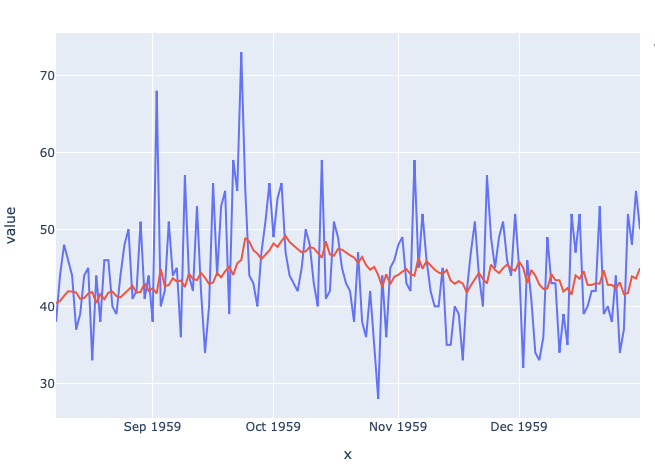
\includegraphics[scale=0.5]{Images/1.1}
			\end{figure}
			\item \textbf{shampo}: SARIMAX. 
			\begin{figure}[H]
				\centering 
				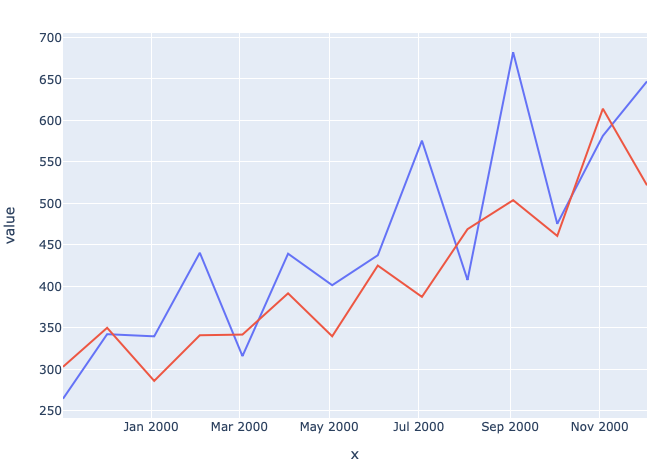
\includegraphics[scale=0.5]{Images/1.2}
			\end{figure}
			\item \textbf{monthly-car-sales}: Prophet. 
			\begin{figure}[H]
				\centering 
				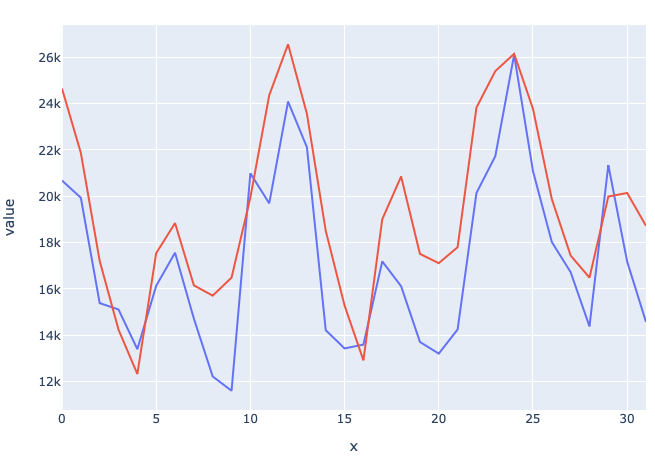
\includegraphics[scale=0.5]{Images/1.3}
			\end{figure}
			\item \textbf{monthly-mean-temps}: Prophet. 
			\begin{figure}[H]
				\centering 
				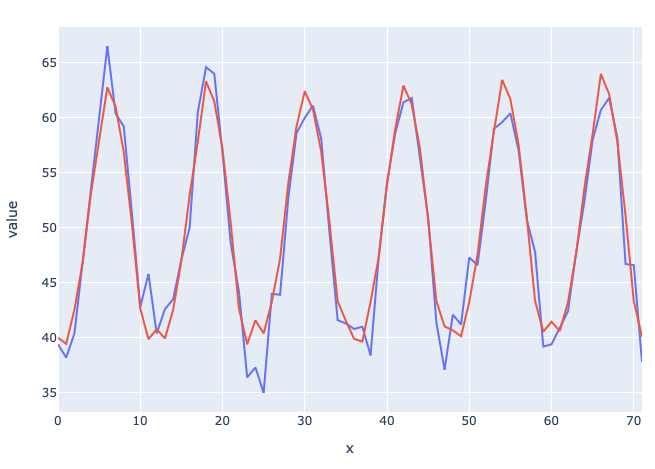
\includegraphics[scale=0.5]{Images/1.4}
			\end{figure}
		\end{enumerate}
	\end{sol}
\end{problema}

%----------------------
\begin{problema}
	¿Qué métodos logran captar mejor las tendencias y las variaciones estacionales? 
	\begin{sol}
		Eso dependerá mucho de la base de datos proporcionada. En resumen, los métodos que mejor capturan las tendencias y variaciones estacionales son: Prophet y redes neuronales. Aunque en algunos casos SARIMAX y Winter-Holt, también resultan muy efectivos.
	\end{sol}
\end{problema}

%----------------------
\begin{problema}
	Generen una tabla comparativa que muestre los RMSE más bajos para cada método con cada conjunto de datos. En la tabla indiquen qué método fue mejor para cada caso de datos.  Por ejemplo:
	\begin{figure}[H]
		\centering
		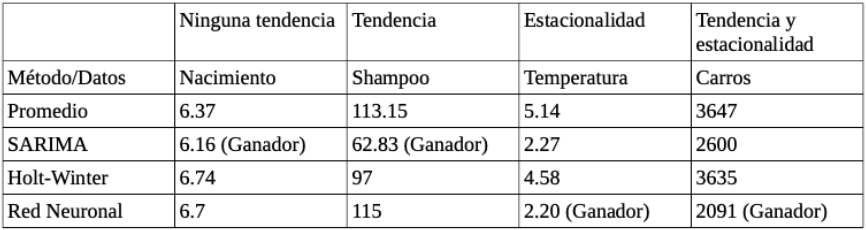
\includegraphics[scale=0.5]{Images/1}
	\end{figure}
\begin{sol}
	Los resultados obtenidos son los siguientes: 
	\begin{table}[H]
		\caption{Comparación de RMSE}
		\label{tab:rmse}
		\resizebox{\columnwidth}{!}{%
		\begin{tabular}{@{}c|cccc@{}}
			\toprule
			\textit{\textbf{\begin{tabular}[c]{@{}c@{}}Conjunto de datos/\\ Método\end{tabular}}} & \textbf{daily-total-female-births} & \textbf{shampoo} & \textbf{monthly-car-sales} & \textbf{monthly-mean-temp} \\ \midrule
			\textbf{Promedio}                                                                     & 7.51                               & 188.54           & 3676.92                    & 5.91                       \\
			\textbf{SARIMAX}                                                                      & {\ul 6.98}                         & {\ul 88.27}      & 3134.12                    & 4.39                       \\
			\textbf{Winter-Holt}                                                                  & 7.21                               & 101.75           & 3706.02                    & 5.33                       \\
			\textbf{Red Neuronal}                                                                 & 8.05                               & 257.61           & 3481.97                    & 5.063                      \\
			\textbf{Prophet}                                                                      & 7.46                               & 304              & {\ul 2839.13}              & {\ul 2.19}                 \\ \bottomrule
		\end{tabular}%
	}
	
	\end{table}
\end{sol}
\end{problema}

%----------------------
\begin{problema}
	Ahora apliquen el FB Prophet con cada uno de los conjuntos de datos. Compare los resultados con los de los métodos anteriores.  ¿Hay algún ganador claro, entre todos los métodos?
	\begin{sol}
		Nuevamente, la respuesta dependerá del conjunto de datos de por sí; en la base de datos de carros y de temperaturas, Prophet es un claro vencedor. Sin embargo, en las primeras dos bases de datos de cumpleaños de mujeres y de shampoo, Prophet se queda bastante rezagado. Así que los mejores algoritmos están entre SARIMAX y Prophet. 
	\end{sol}
\end{problema}


%----------------------
\begin{problema}
	 Escriban sus conclusiones sobre lo aprendido en este módulo sobre series de tiempo.  ¿Cuál es el mejor procedimiento para resolver un problema de predicción de series de tiempo?  
	 \begin{sol}
	 	Algunas conclusiones:
	 	\begin{enumerate}
	 		\item No existe un método totalmente dominante, ya que todos tienen fluctuaciones y principalmente sus rendimientos se basan en la base de datos proporcionada. 
	 		\item Para comprender mejor que algoritmo es mejor es necesario tener un conocimiento teórico del tema, ya que existen diversidad de parámetros que poseen los métodos que podrían ser utilizados y resultar bastante efectivos.
	 		\item El modelo de SARIMAX pareciera ser bastante efectivo al colocarle sus parámetros correctos por medio del Grid Search, por lo cual es de suma utilidad implementar este método.
	 	\end{enumerate}
	 \end{sol}
\end{problema}



%---------------------------
\bibliographystyle{apa}
\bibliography{referencias.bib}

\end{document}